\subsubsection{HandBag Model}
The production of the \piz meson in photon-proton reactions, for incoming photon beam energies greater than 2.8~GeV, can considered to be a hard exclusive reaction. One approach to study the \piz photoproduction, is use the handbag model. In the handbag approach, the reaction is factorized into two parts. The first part is when one quark from the incoming and one from the outgoing nucleon participate in the hard sub-process. This hard sub-process is achieved when the incident photon excites a quark, since quarks are bound quantum particles, the excited quark produces a jet of quarks that form the meson and then de-excites back into the nucleon. This is calculable using pQCD. The second part ,the soft part, consists of all the other quarks that are spectators and can be described in terms of GPDs~\cite{key1, key2,Rad1996, Diehl}. The handbag mechanism is applicable when the Mandelstam variables, $s$, $t$, $u$, are large as compared to a hadronic scale of order 1 GeV . In Ref.~\cite{Huang2000} a model, derived from the handbag approach, has been applied to predict angular dependence of scaled photoproduction cross section of \piz and is illustrated in Fig.~\ref{fig:pi0_handbag}. The handbag model calculations by Kroll \textit{et al.}~\cite{Huang2000} does not agree with the measurement obtained by \g12.
\begin{figure}[h]
	\centerline{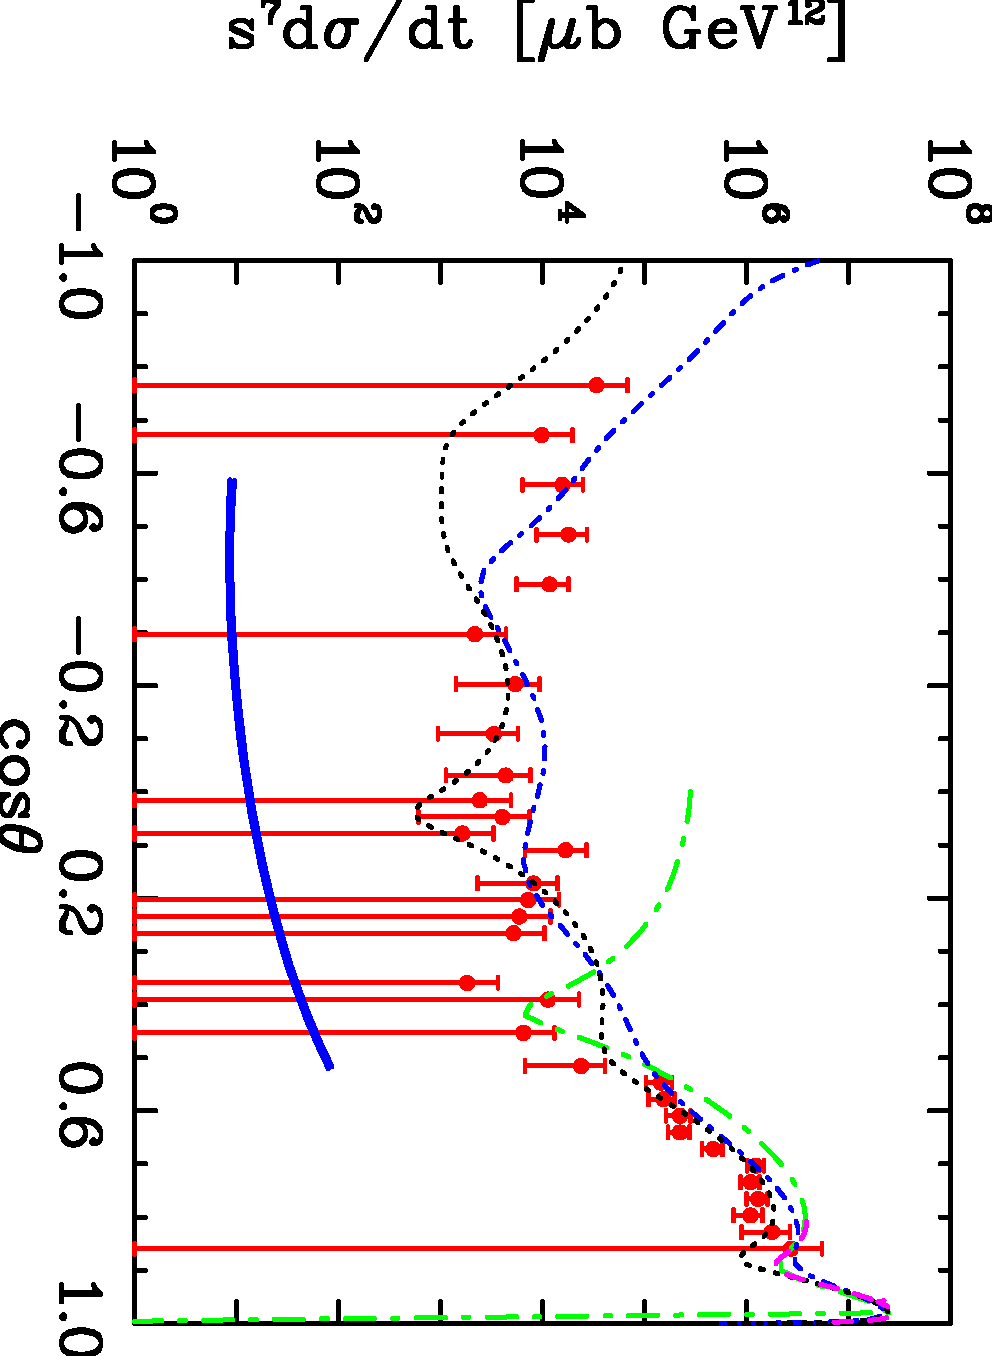
\includegraphics[width=200 pt]{\figures/analysis/DSG/kroll-eps-converted-to.pdf}}
	\caption{Comparison of the $\pi^0$ differential cross section  photoproduction data to \abbr{GDP} handbag model. Experimental data at $s$ = 11.08~GeV$^2$ are from the current (red filled circles). The theoretical prediction at $s$ = 10~GeV$^2$ by Kroll \textit{et al.}~\protect\cite{Huang2000} is given by blue solid line.}
	\label{fig:pi0_handbag}
\end{figure}